\chapter{Conception}

\section{Introduction}

Ce chapitre présente la phase de conception technique de l'application. Cette étape cruciale permet de traduire les besoins fonctionnels identifiés précédemment en une architecture logicielle cohérente. À travers une modélisation utilisant le langage UML (Unified Modeling Language), nous détaillerons les interactions entre les différents acteurs et le système via les cas d'utilisation, la structure statique des données à travers le diagramme de classes, ainsi que la dynamique des processus métiers au moyen des diagrammes de séquences.

\clearpage
\section{Diagramme de Cas d'Utilisation Général}

\begin{figure}[H]
  \centering
  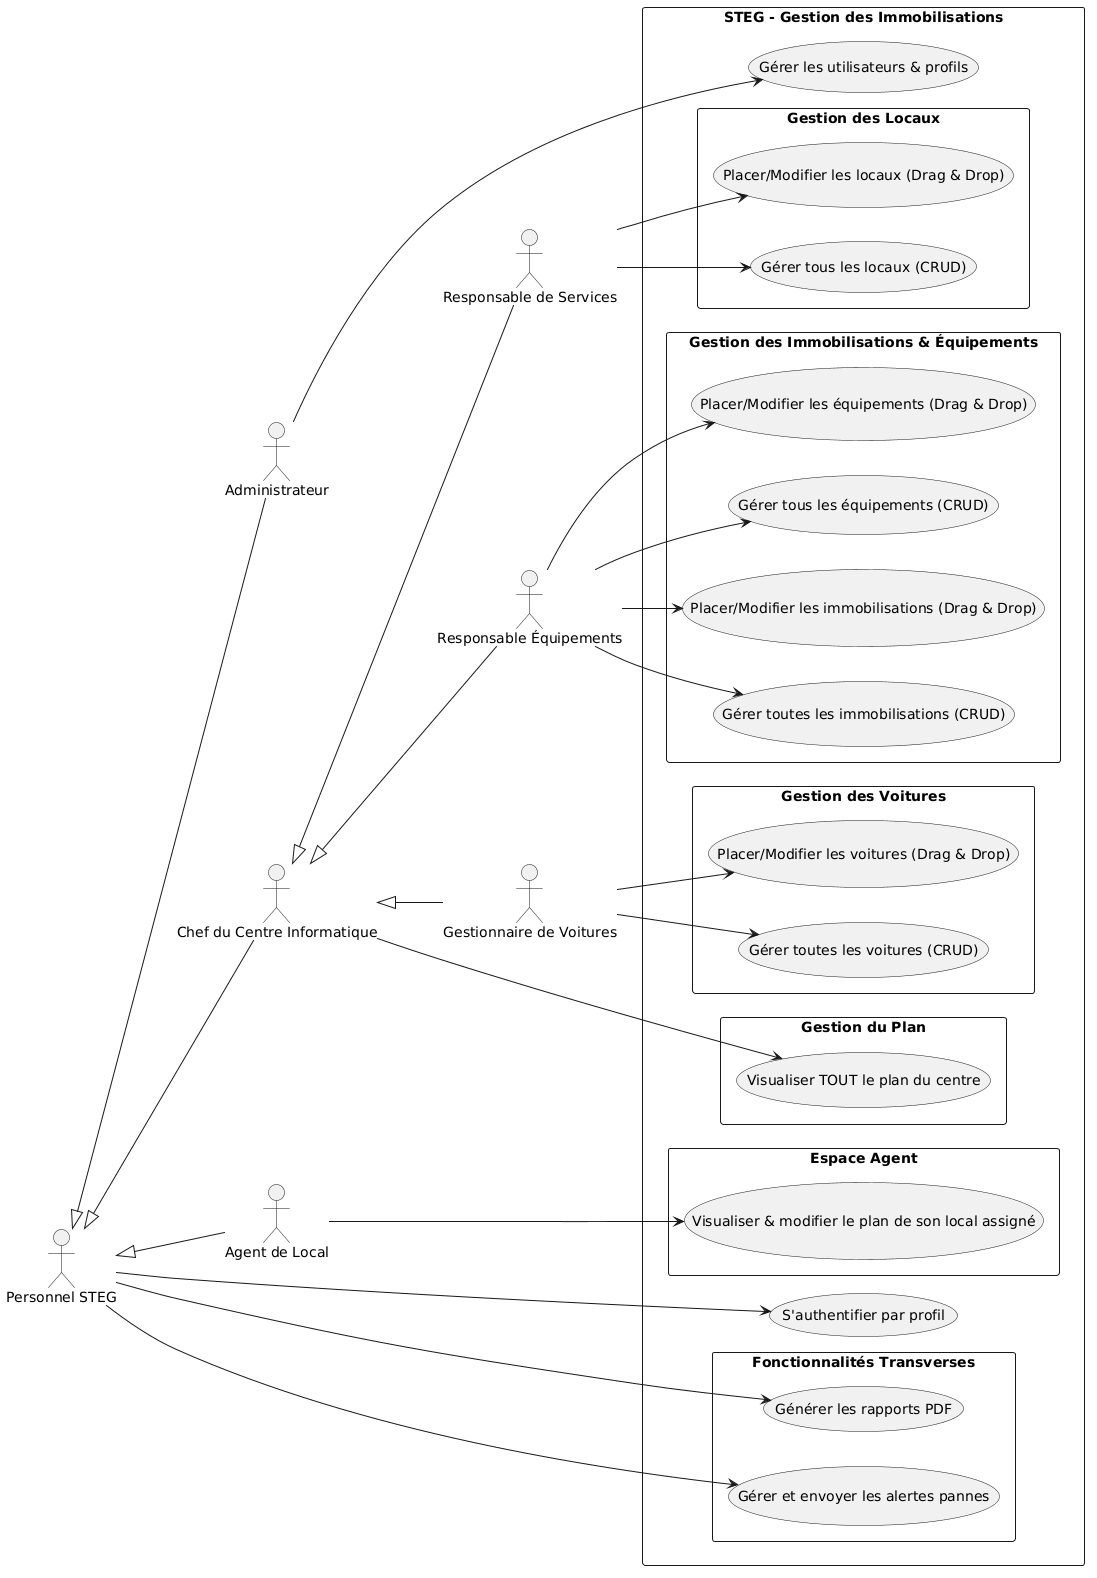
\includegraphics[width=\textwidth,height=0.75\textheight,keepaspectratio]{../../assets/use_case_diagram.png}
  \caption{Diagramme de cas d'utilisation général}
  \label{fig:use_case}
\end{figure}

\clearpage
\section{Diagramme de Classes Général}

\begin{figure}[H]
  \centering
  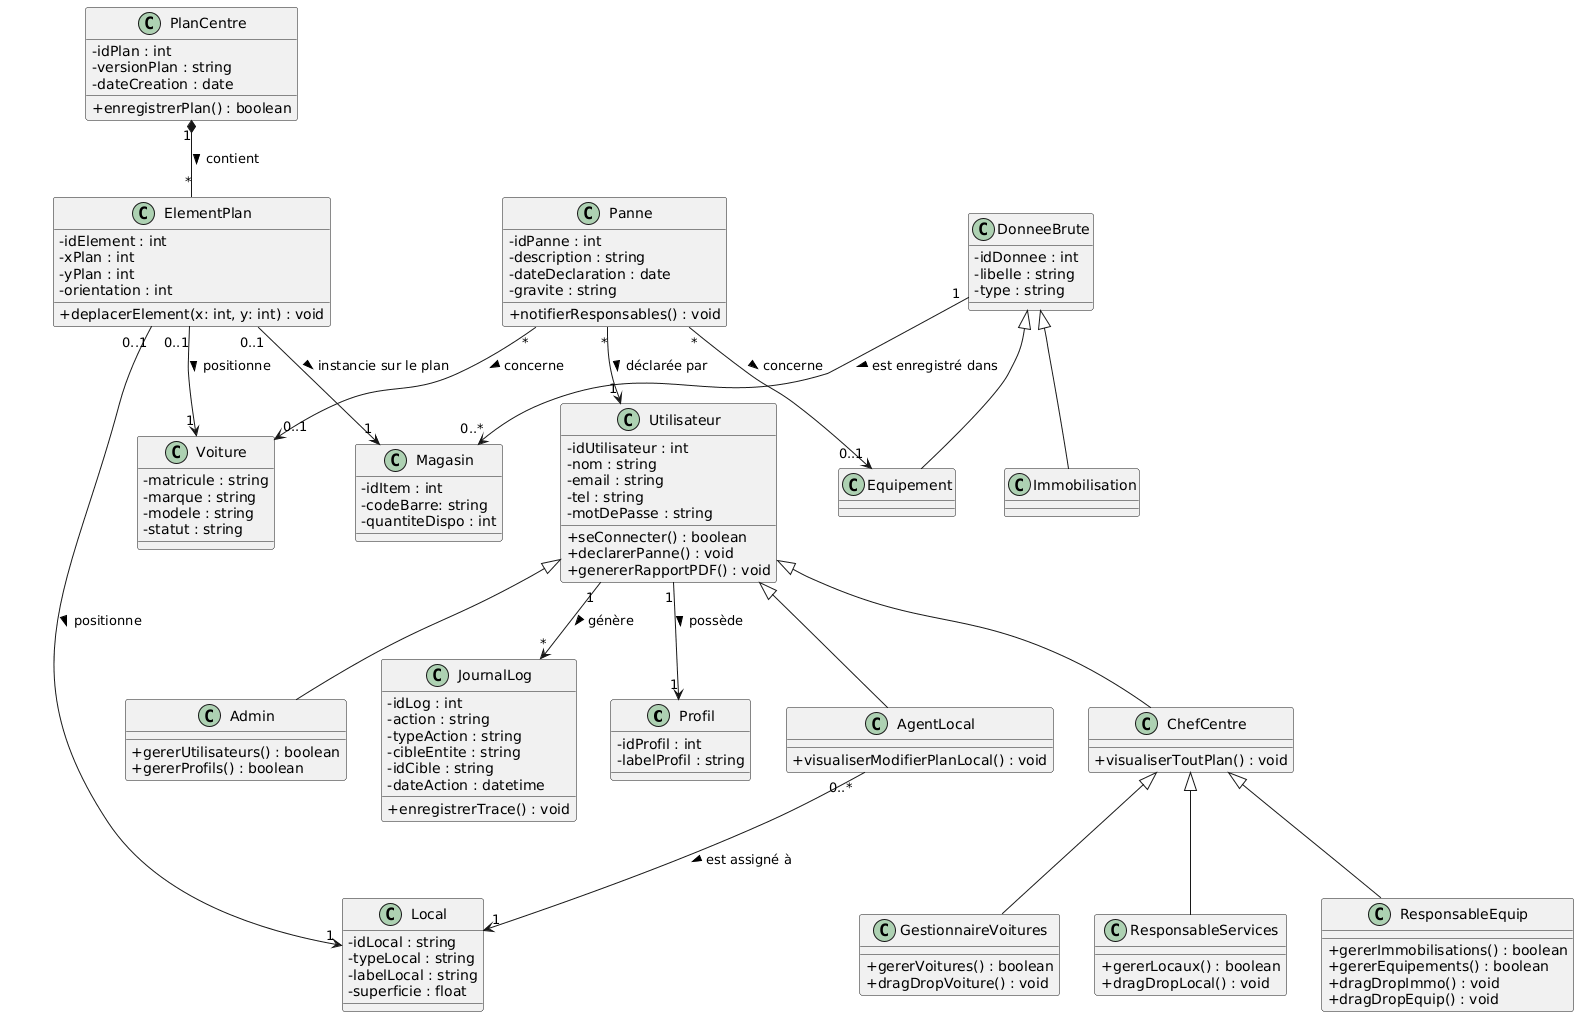
\includegraphics[width=\textwidth,height=0.75\textheight,keepaspectratio]{../../assets/class_diagram.png}
  \caption{Diagramme de classes général}
  \label{fig:class_diagram}
\end{figure}

\clearpage
\section{Diagramme de Séquences}

\subsection{Scénario d'Authentification (UC\_Auth)}

Le processus d'authentification représente le point d'entrée sécurisé de l'application. La cinématique ci-dessous détaille la vérification des identifiants ainsi que l'affectation dynamique de l'espace de travail en fonction du profil récupéré depuis la base de données.

\begin{figure}[H]
  \centering
  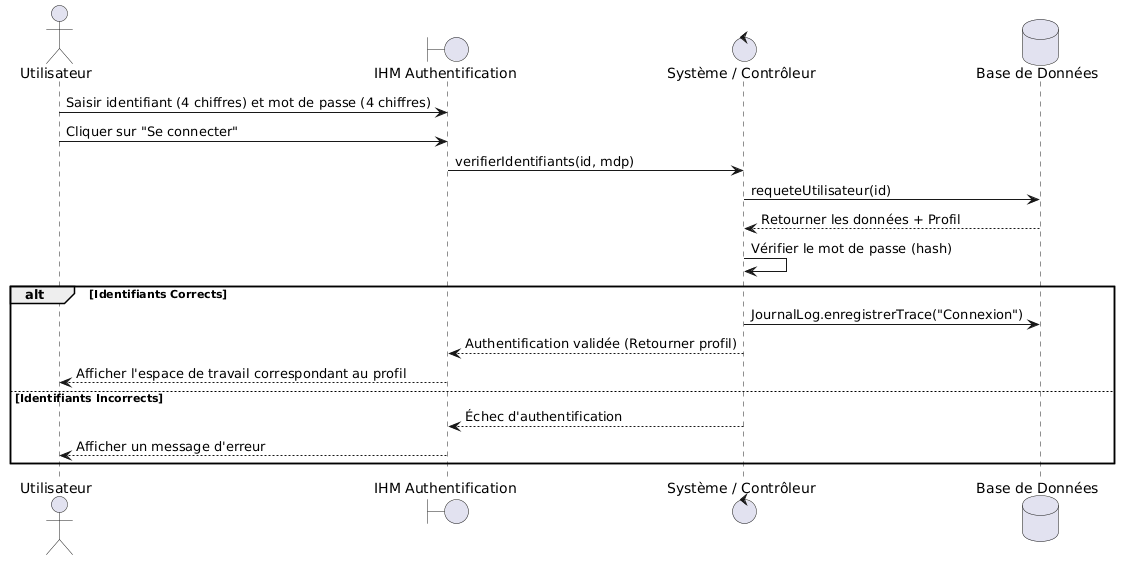
\includegraphics[width=\textwidth,height=0.65\textheight,keepaspectratio]{../../assets/seq_auth.png}
  \caption{Diagramme de séquence - Authentification par profil}
  \label{fig:seq_auth}
\end{figure}

\clearpage
\subsection{Scénario de Gestion des Utilisateurs (UC\_Admin\_System)}

Réservé exclusivement au profil Administrateur, ce cas d'utilisation décrit la logique de persistance lors de la création d'un nouveau compte utilisateur, incluant la vérification d'unicité de l'identifiant et l'écriture systématique dans le journal de traçabilité.

\begin{figure}[H]
  \centering
  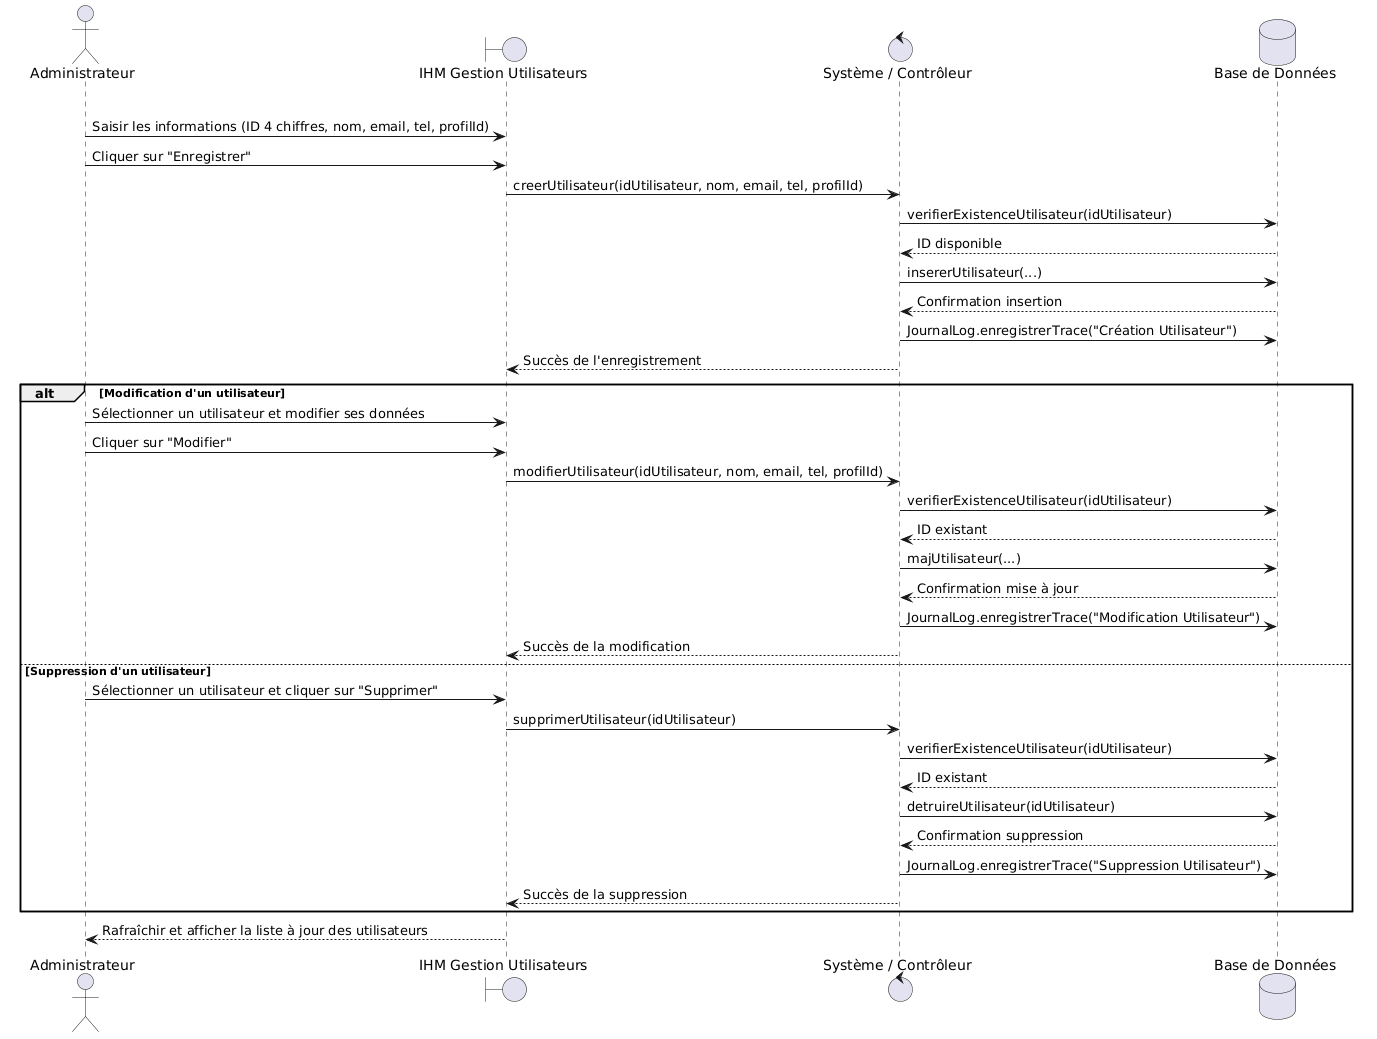
\includegraphics[width=\textwidth,height=0.65\textheight,keepaspectratio]{../../assets/seq_admin.png}
  \caption{Diagramme de séquence - Gestion des utilisateurs et profils}
  \label{fig:seq_admin}
\end{figure}

\clearpage
\subsection{Scénario de Visualisation du Plan}

Cette cinématique met en évidence le filtrage des données selon les privilèges de l'acteur connecté. Là où le Chef du Centre obtient une vue globale de l'infrastructure, l'Agent de Local ne reçoit que les éléments géographiques restreints à sa zone d'affectation.

\begin{figure}[H]
  \centering
  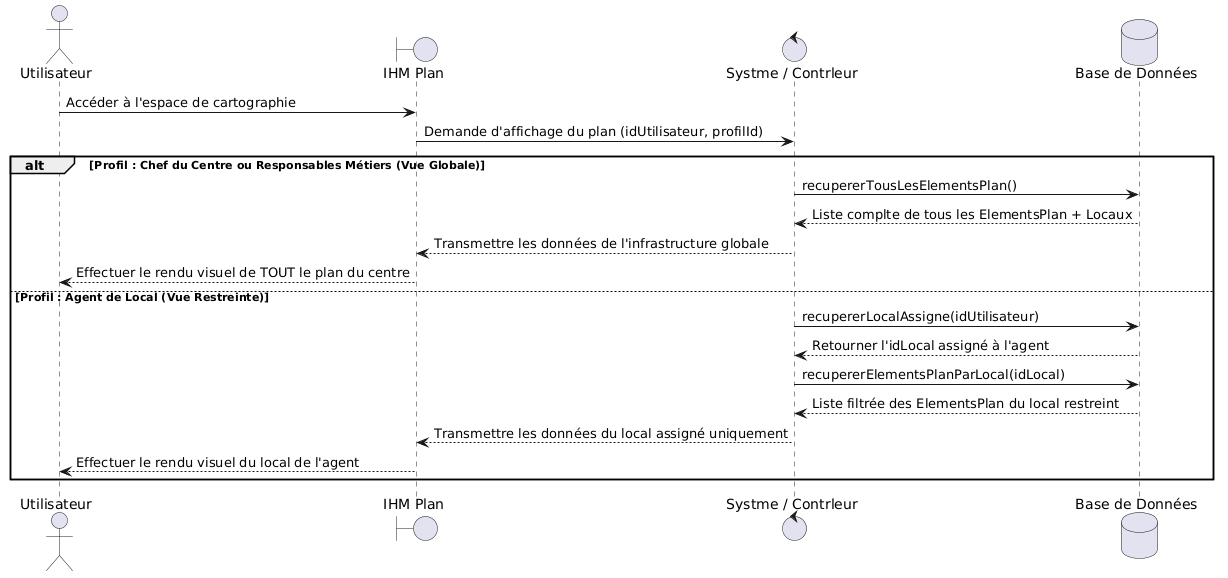
\includegraphics[width=\textwidth,height=0.65\textheight,keepaspectratio]{../../assets/seq_voir_plan.png}
  \caption{Diagramme de séquence - Visualisation du plan}
  \label{fig:seq_voir_plan}
\end{figure}

\clearpage
\subsection{Scénario de Gestion et d'Enregistrement Intermédiaire (UC\_CRUD\_Equip)}

Ce diagramme illustre la règle métier stricte du système : toute donnée brute d'équipement ou d'immobilisation créée par le responsable doit obligatoirement être enregistrée au sein de la table magasin avant de pouvoir être exploitée lors de la phase de cartographie.

\begin{figure}[H]
  \centering
  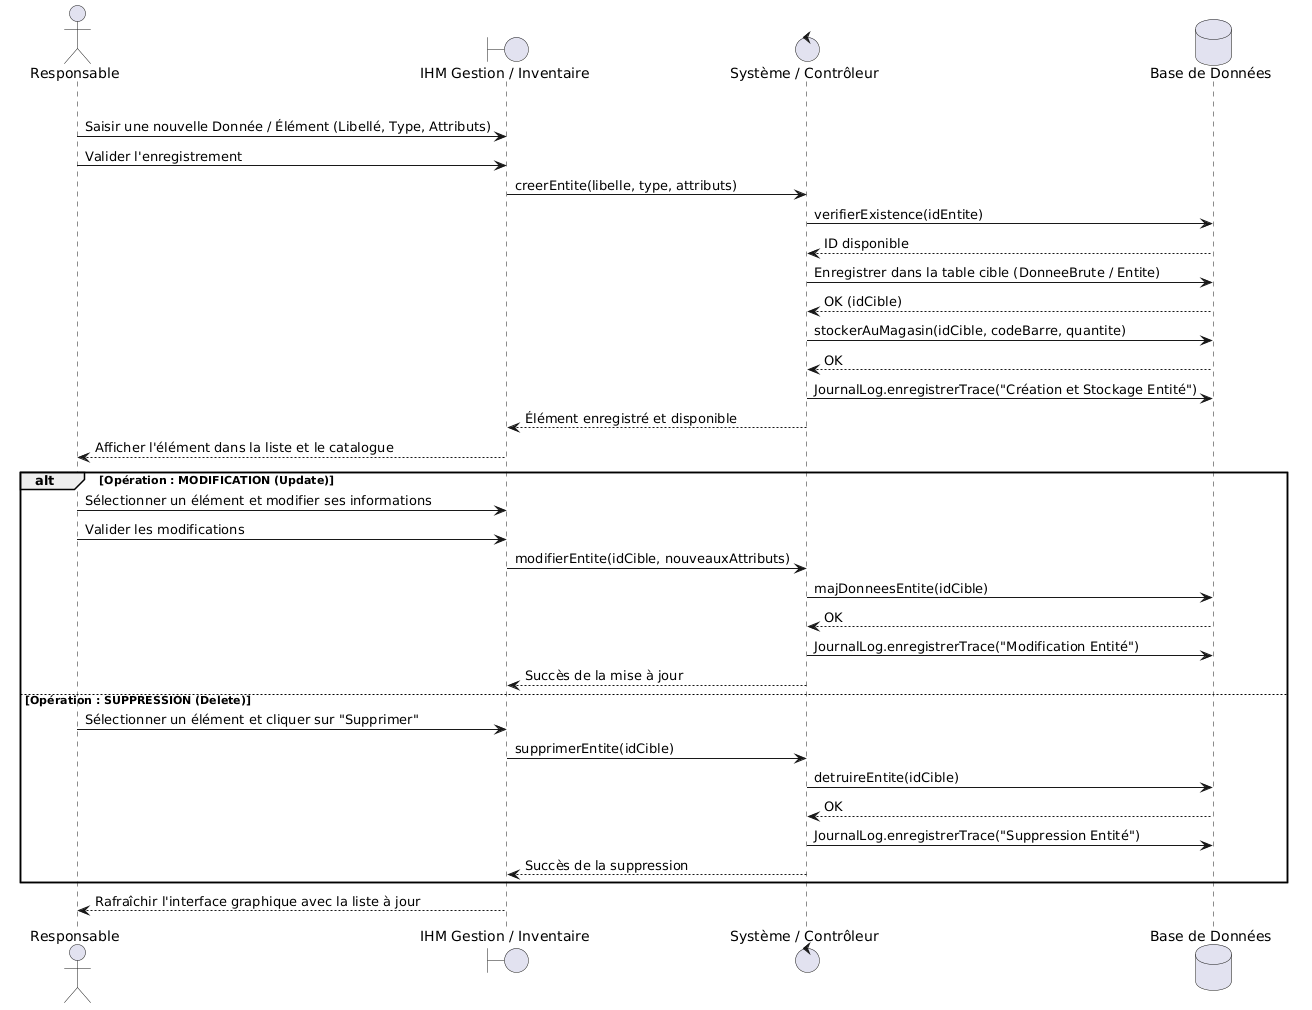
\includegraphics[width=\textwidth,height=0.65\textheight,keepaspectratio]{../../assets/seq_crud.png}
  \caption{Diagramme de séquence - Enregistrement en magasin}
  \label{fig:seq_crud_equip}
\end{figure}

\clearpage
\subsection{Scénario de Placement Spatial par Glisser-Déposer (UC\_DragDrop\_Immo)}

L'aspect dynamique du positionnement graphique traduit l'interaction de l'utilisateur avec l'interface interactive. Le contrôleur instancie un élément de plan aux coordonnées $(X, Y)$ spécifiées et met à jour la base de données en temps réel.

\begin{figure}[H]
  \centering
  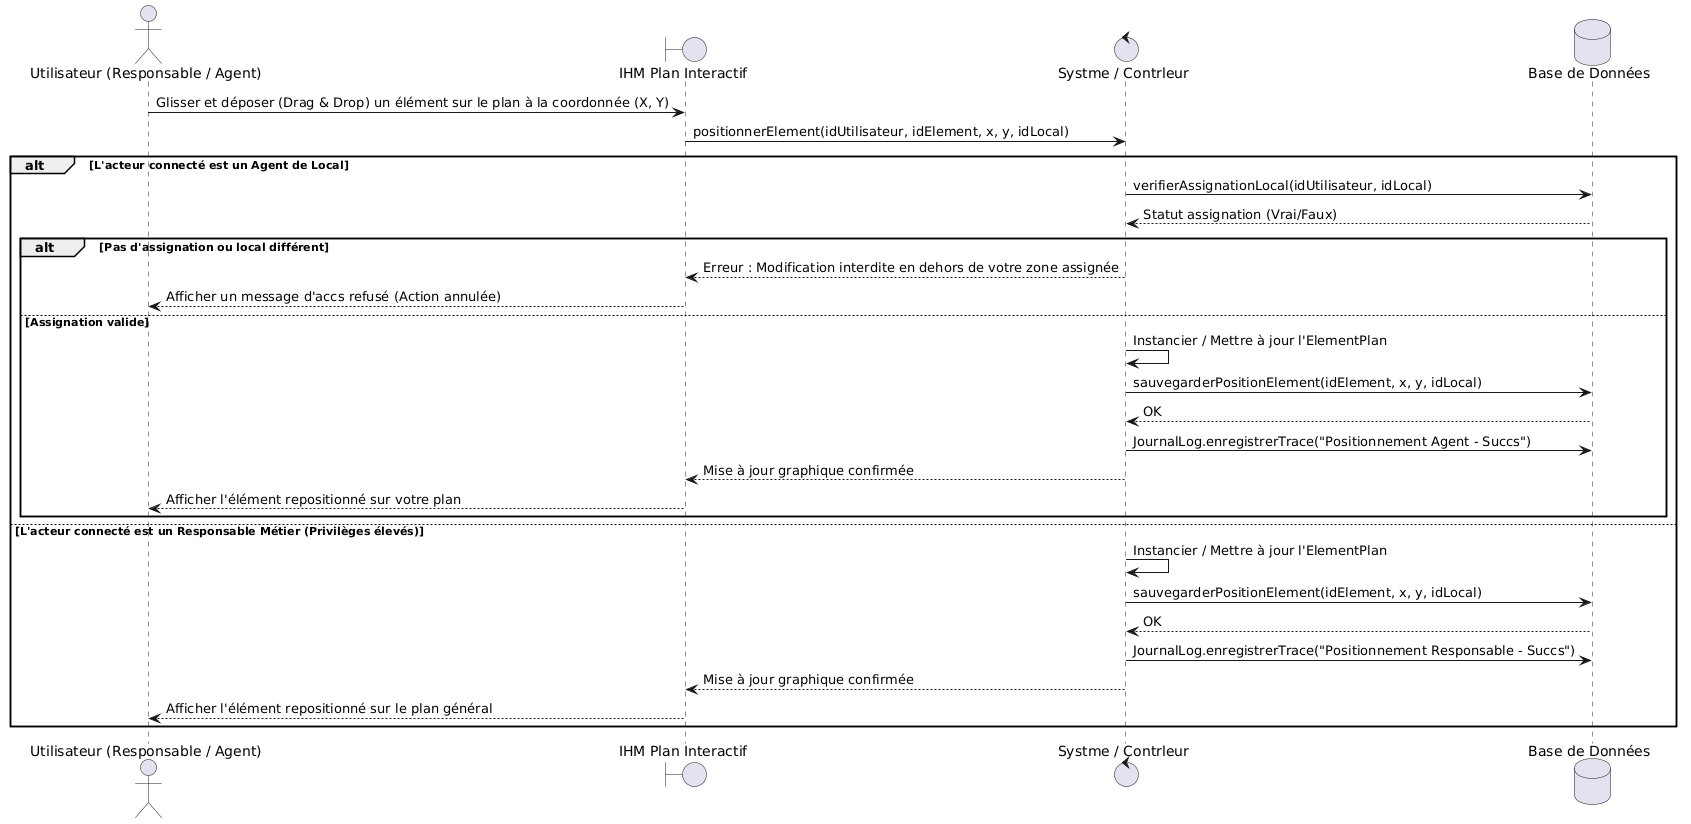
\includegraphics[width=\textwidth,height=0.65\textheight,keepaspectratio]{../../assets/seq_drag_drop.png}
  \caption{Diagramme de séquence - Placement des éléments sur le plan}
  \label{fig:seq_drag_drop}
\end{figure}

\clearpage
\subsection{Scénario de Gestion et de Notification des Pannes (UC\_Alertes)}

Le processus de déclaration d'une panne déclenche un mécanisme d'aiguillage automatique. Selon la nature de l'entité ciblée (matériel technique ou véhicule), le système identifie et notifie le responsable métier concerné tout en historisant l'incident.

\begin{figure}[H]
  \centering
  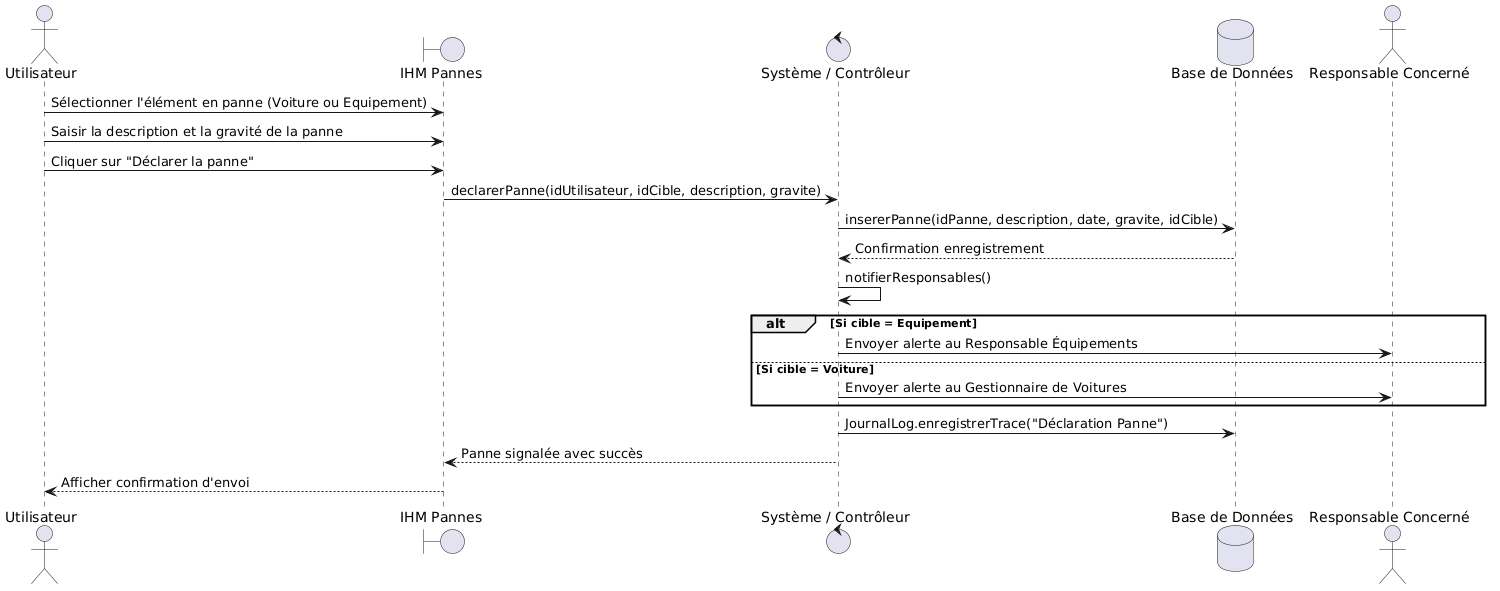
\includegraphics[width=\textwidth,height=0.65\textheight,keepaspectratio]{../../assets/seq_alertes.png}
  \caption{Diagramme de séquence - Déclaration et routage d'une alerte panne}
  \label{fig:seq_alertes}
\end{figure}

\clearpage
\subsection{Scénario de Génération Globale de Rapports (UC\_PDF)}

Conformément à l'extension des droits d'accès à l'ensemble du personnel de la STEG, ce scénario décrit la collecte transverse des données applicatives, leur compilation au format PDF et l'interrogation du journal de log à des fins d'audit de l'action.

\begin{figure}[H]
  \centering
  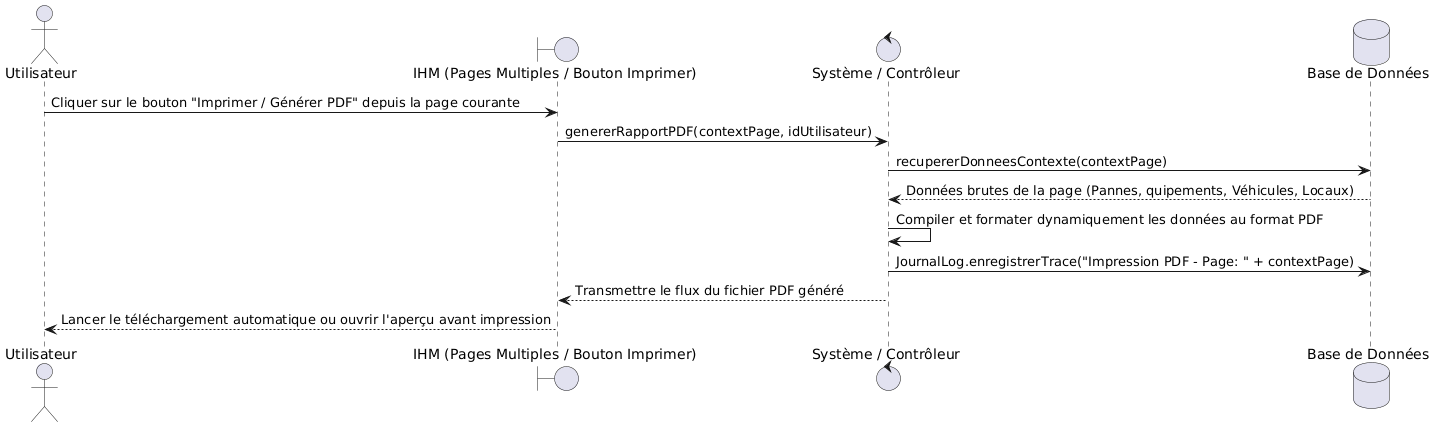
\includegraphics[width=\textwidth,height=0.65\textheight,keepaspectratio]{../../assets/seq_pdf.png}
  \caption{Diagramme de séquence - Génération de rapports PDF}
  \label{fig:seq_pdf}
\end{figure}

\clearpage
\section{Conclusion du Chapitre}

La phase de modélisation présentée dans ce chapitre a permis de figer l'ensemble des interactions et des structures nécessaires à la réalisation de l'application de gestion des immobilisations de la STEG. L'alignement rigoureux entre les cas d'utilisation, l'architecture statique des classes et la cinématique des diagrammes de séquences assure une transition fluide et sécurisée vers la phase de développement et d'implémentation technique.